\documentclass[conference]{IEEEtran}
\usepackage[T1]{fontenc}
\usepackage{amsmath}
\usepackage{booktabs}
\usepackage{graphicx}
\usepackage{xcolor}
\usepackage{tikz}
\usetikzlibrary{arrows.meta,positioning,calc}
\usepackage{balance}
\usepackage[hidelinks]{hyperref}
\hypersetup{pdftitle={KVFold: Expanding Cache Capacity for LLM Agents with Lossless Compression},
            pdfsubject={ICDE demonstration working draft, version 8}}
\definecolor{fpInk}{HTML}{172634}
\definecolor{fpBlue}{HTML}{1D62D0}
\definecolor{fpTeal}{HTML}{007E6A}
\definecolor{fpOrange}{HTML}{D96C05}
\definecolor{fpPurple}{HTML}{735892}
\tikzset{
  fpbox/.style={draw,rounded corners=2pt,align=center,inner sep=5pt,
                minimum height=0.73cm,line width=0.65pt},
  fparrow/.style={-{Stealth[length=1.7mm]},line width=0.8pt,draw=fpInk},
  fpboth/.style={{Stealth[length=1.7mm]}-{Stealth[length=1.7mm]},
                 line width=0.8pt,draw=fpInk}
}
\title{KVFold: Expanding Cache Capacity for \mbox{LLM Agents} with Lossless Compression}
\author{\IEEEauthorblockN{Working draft}
\IEEEauthorblockA{Author information to be supplied}}
\raggedbottom
\begin{document}
\maketitle

\begin{abstract}
LLM agents often reuse long prompt prefixes as they continue a task or
resume a session. Caching the corresponding key/value (KV) states avoids
repeated prefill, but cache capacity limits how many requests can run
concurrently and how much history can be retained. KVFold uses lossless
exponent coding to fit more KV into GPU memory and external storage.
Pool mode stores FragPack records on the GPU, decoding them into BF16 for
FlashAttention-3 during prefill and within a fused attention kernel during
decode. Tier mode uses a separate record
format in LMCache and leaves the GPU cache layout and attention
implementation unchanged. In recorded AgentX runs with a fixed 54~GiB KV
budget per GPU, pool mode increases usable capacity from 1.18M to 1.59M
tokens. Visitors can extend and edit a coding-agent prompt to inspect
prefix reuse and KV reconstruction, then explore recorded results showing
how the additional capacity affects concurrent requests and returning
sessions.
\end{abstract}

\section{Introduction}
Consider a coding agent investigating a timeout. Its prompt includes
repository context, a bug report, and the investigation history. When the
user follows the diagnosis with a request for a regression test, most of
the prompt remains unchanged. Prefix caching lets the engine reuse the
keys and values already computed for this shared context, avoiding repeated
prefill. vLLM stores KV in paged blocks~\cite{vllm}, while LMCache retains
reusable prefixes in DRAM and NVMe across requests~\cite{lmcache}.

For Qwen3-30B-A3B, each cached token requires 96~KiB of BF16 KV across all
layers. With many concurrent sessions, requests may have to wait for free
GPU blocks even when their prefixes are available in external storage.
Moving inactive histories to external tiers relieves GPU memory pressure,
but those tiers can also fill up. When a session resumes after its prefix
has been evicted, the engine must recompute that prefix. Cache capacity
thus limits both request concurrency and the amount of history available
for reuse.

KVFold uses lossless compression to fit more KV into the available GPU
memory and external storage. The codec preserves each BF16 value's low
byte, assigns short codes to frequent high-byte values, and uses escapes
for the remaining values. Unlike quantization methods such as
KIVI~\cite{kivi} or lossy context codecs such as CacheGen~\cite{cachegen},
it reconstructs the original KV bits. The main \emph{pool mode} stores
completed GPU blocks as FragPack records. During prefill, KVFold gathers
and decodes the context's KV into a BF16 workspace for FlashAttention-3
(FA3)~\cite{fa3}. During decode, it reconstructs operands within a fused
attention kernel. An alternative \emph{tier mode} stores compressed KV in
LMCache while retaining the native GPU cache layout and attention
implementation. Both modes share the coding principle and offline
calibration, but use different record formats for attention and external
storage.

The demonstration follows the agent as it continues a task, runs alongside
other sessions, and resumes an earlier investigation. Interactive requests
show prefix reuse, external restoration, and KV byte checks.
Recorded AgentX workloads~\cite{agentx} illustrate the effect at scale:
with a 54~GiB KV budget per GPU, pool mode holds 1.59M tokens compared
with 1.18M for the uncompressed baseline. With admission capped at
12 requests, mean engine time to first token (TTFT) falls from 5.16 to
1.94~s, excluding time spent waiting at the proxy.

\begin{figure*}[t]
\centering
% KVFold architecture, manuscript version 5.
% Topology: industry.pdf, Sections III--VI, and manuscript version 3.
% Native vector primitives; oblique depth denotes pages, chips and devices,
% not measured capacity. Blue = FragPack payload; orange = BF16/attention;
% teal = external-cache devices and tier payload. The lanes are alternatives.
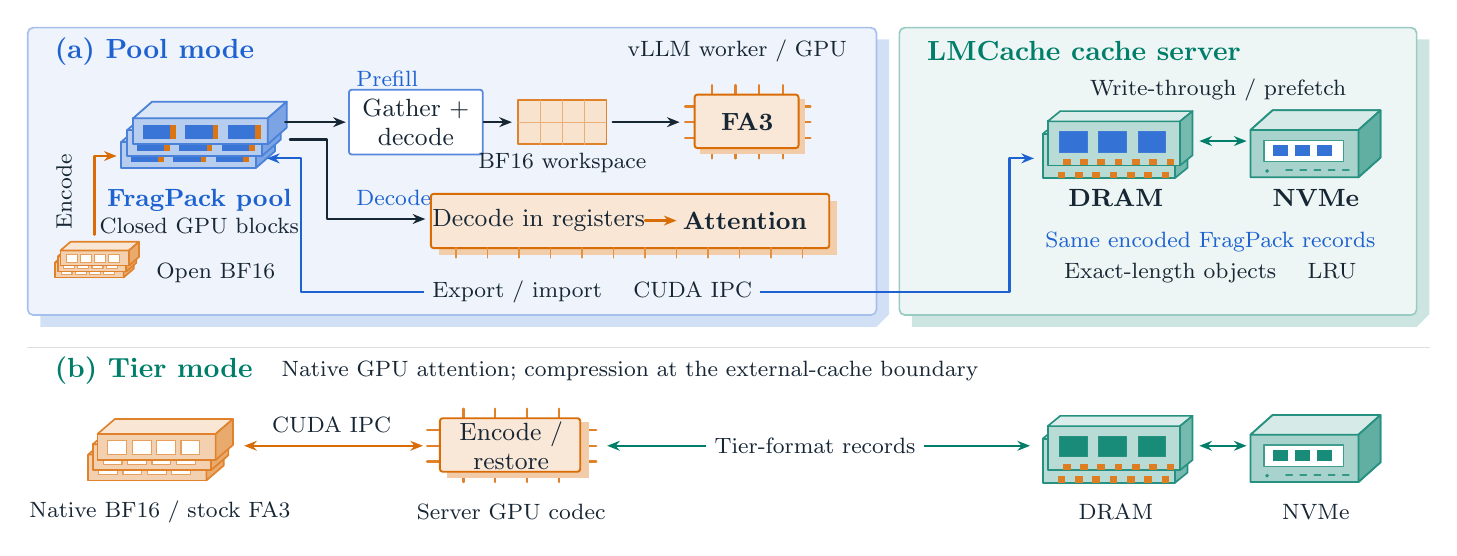
\begin{tikzpicture}[x=1cm,y=1cm,text=fpInk,
    font=\fontsize{9}{10.5}\selectfont,
    line join=round,line cap=round,
    flow/.style={-{Stealth[length=1.6mm,width=1.25mm]},line width=.8pt,draw=fpInk},
    transfer/.style={{Stealth[length=1.6mm,width=1.25mm]}-{Stealth[length=1.6mm,width=1.25mm]},line width=.8pt,draw=fpBlue},
    smalltext/.style={font=\fontsize{8}{9}\selectfont},
    pics/packed/.style={code={
      \foreach \z in {0,.15,.30} {
        \begin{scope}[shift={(.5*\z,\z)}]
          \draw[fpBlue!80,line width=.65pt,fill=fpBlue!32]
            (-.91,-.13) rectangle (.80,.20);
          \draw[fpBlue!80,line width=.65pt,fill=fpBlue!16]
            (-.91,.20) -- (-.67,.41) -- (1.04,.41) -- (.80,.20) -- cycle;
          \draw[fpBlue!80,line width=.65pt,fill=fpBlue!58]
            (.80,-.13) -- (1.04,.08) -- (1.04,.41) -- (.80,.20) -- cycle;
          \foreach \x in {-.79,-.25,.29} {
            \fill[fpBlue!88] (\x,-.06) rectangle +( .35,.17);
            \fill[fpOrange!94] (\x+.35,-.06) rectangle +(.07,.17);
          }
        \end{scope}
      }
    }},
    pics/native/.style={code={
      \foreach \z in {0,.13,.26} {
        \begin{scope}[shift={(.45*\z,\z)}]
          \draw[fpOrange!85,line width=.6pt,fill=fpOrange!32]
            (-.83,-.21) rectangle (.67,.12);
          \draw[fpOrange!85,line width=.6pt,fill=fpOrange!17]
            (-.83,.12) -- (-.61,.31) -- (.89,.31) -- (.67,.12) -- cycle;
          \draw[fpOrange!85,line width=.6pt,fill=fpOrange!58]
            (.67,-.21) -- (.89,-.02) -- (.89,.31) -- (.67,.12) -- cycle;
          \foreach \x in {-.70,-.39,-.08,.23} {
            \draw[fpOrange!65,fill=white,line width=.4pt]
              (\x,-.14) rectangle +(.24,.18);
          }
        \end{scope}
      }
    }},
    pics/chip/.style={code={
      \foreach \x in {-.45,-.15,.15,.45} {
        \draw[fpOrange!85,line width=.9pt] (\x,-.46) -- (\x,-.34);
        \draw[fpOrange!85,line width=.9pt] (\x,.34) -- (\x,.47);
      }
      \foreach \y in {-.20,0,.20} {
        \draw[fpOrange!85,line width=.9pt] (-.79,\y) -- (-.65,\y);
        \draw[fpOrange!85,line width=.9pt] (.65,\y) -- (.80,\y);
      }
      \fill[fpOrange!35] (-.60,-.41) rectangle (.73,.30);
      \draw[fpOrange,line width=.7pt,fill=fpOrange!16,rounded corners=1pt]
        (-.67,-.33) rectangle (.65,.35);
    }},
    pics/dram/.style={code={
      \foreach \z in {0,.16} {
        \begin{scope}[shift={(.40*\z,\z)}]
          \draw[fpTeal!85,line width=.65pt,fill=fpTeal!28]
            (-.84,-.25) rectangle (.84,.31);
          \draw[fpTeal!85,line width=.6pt,fill=fpTeal!14]
            (-.84,.31) -- (-.68,.44) -- (1.0,.44) -- (.84,.31) -- cycle;
          \draw[fpTeal!85,line width=.6pt,fill=fpTeal!54]
            (.84,-.25) -- (1.0,-.12) -- (1.0,.44) -- (.84,.31) -- cycle;
          \foreach \x in {-.69,-.19,.31} {
            \draw[fpPayload!85,line width=.4pt,fill=fpPayload!90]
              (\x,-.08) rectangle +(.35,.26);
          }
          \foreach \x in {-.65,-.43,-.21,.01,.23,.45,.67} {
            \fill[fpOrange!88] (\x,-.25) rectangle +(.10,.08);
          }
        \end{scope}
      }
    }},
    pics/nvme/.style={code={
      \draw[fpTeal!85,line width=.65pt,fill=fpTeal!34]
        (-.72,-.24) -- (.65,-.24) -- (.93,.01) -- (.93,.61)
        -- (-.44,.61) -- (-.72,.36) -- cycle;
      \draw[fpTeal!85,line width=.65pt,fill=fpTeal!16]
        (-.72,.36) -- (-.44,.61) -- (.93,.61) -- (.65,.36) -- cycle;
      \draw[fpTeal!85,line width=.65pt,fill=fpTeal!62]
        (.65,-.24) -- (.93,.01) -- (.93,.61) -- (.65,.36) -- cycle;
      \draw[fpTeal!75,line width=.5pt,fill=white]
        (-.55,-.04) rectangle (.46,.23);
      \foreach \x in {-.44,-.16,.12} {
        \fill[fpPayload!90] (\x,.025) rectangle +(.20,.14);
      }
      \fill[fpTeal!85] (-.51,-.16) circle (.025);
      \foreach \x in {-.27,-.09,.09,.27,.45} {
        \draw[fpTeal!80,line width=.55pt] (\x,-.15) -- +( .08,0);
      }
    }}]
  \path[use as bounding box] (0,0) rectangle (17.8,6.35);
  \colorlet{fpPayload}{fpBlue}

  % Raised host regions: the main reader path stays inside the vLLM worker.
  \fill[fpBlue!20] (.16,2.55) -- (10.78,2.55) -- (10.94,2.71)
    -- (10.94,6.20) -- (.16,6.20) -- cycle;
  \fill[fpBlue!7,draw=fpBlue!40,line width=.6pt,rounded corners=2pt]
    (0,2.70) rectangle (10.78,6.35);
  \fill[fpTeal!20] (11.23,2.55) -- (17.64,2.55) -- (17.80,2.71)
    -- (17.80,6.20) -- (11.23,6.20) -- cycle;
  \fill[fpTeal!7,draw=fpTeal!40,line width=.6pt,rounded corners=2pt]
    (11.07,2.70) rectangle (17.64,6.35);
  \node[anchor=west,font=\fontsize{10}{11}\selectfont\bfseries,text=fpBlue]
    at (.22,6.05) {(a) Pool mode};
  \node[anchor=east,smalltext] at (10.53,6.05) {vLLM worker / GPU};
  \node[anchor=west,font=\fontsize{10}{11}\selectfont\bfseries,text=fpTeal]
    at (11.30,6.05) {LMCache cache server};

  % Persistent compressed records and writable, still-open BF16 storage.
  \pic at (2.10,4.70) {packed};
  \node[font=\fontsize{9}{10}\selectfont\bfseries,text=fpBlue]
    at (2.18,4.16) {FragPack pool};
  \node[smalltext] at (2.18,3.84) {Closed GPU blocks};
  \pic[scale=.58] at (.83,3.30) {native};
  \node[smalltext,anchor=west] at (1.51,3.23) {Open BF16};
  \draw[flow,draw=fpOrange] (.85,3.72) -- (.85,4.72) -- (1.13,4.72);
  \node[smalltext,rotate=90,fill=fpBlue!7,inner sep=2pt]
    at (.46,4.27) {Encode};

  % Prefill explicitly materializes BF16 before unchanged FA3.
  \node[smalltext,text=fpBlue,anchor=west] at (4.05,5.70) {Prefill};
  \draw[flow] (3.27,5.15) -- (4.04,5.15);
  \node[draw=fpBlue!75,fill=white,line width=.65pt,rounded corners=1pt,
    minimum width=1.70cm,minimum height=.64cm,align=center]
    (gather) at (4.93,5.15) {Gather +\\decode};
  \draw[flow] (gather.east) -- (6.15,5.15);
  \draw[fpOrange!85,fill=fpOrange!19,line width=.55pt]
    (6.23,4.87) rectangle (7.35,5.43);
  \foreach \x in {6.51,6.79,7.07}
    \draw[fpOrange!55,line width=.45pt] (\x,4.87) -- (\x,5.43);
  \draw[fpOrange!55,line width=.45pt] (6.23,5.15) -- (7.35,5.15);
  \node[smalltext] at (6.79,4.63) {BF16 workspace};
  \draw[flow] (7.43,5.15) -- (8.28,5.15);
  \pic at (9.14,5.15) {chip};
  \node[font=\fontsize{9}{10}\selectfont\bfseries] at (9.14,5.15) {FA3};

  % The decode alternative reconstructs operands inside the attention kernel.
  \draw[flow] (3.33,4.93) -- (3.80,4.93) -- (3.80,3.92) -- (5.05,3.92);
  \node[smalltext,anchor=west,text=fpBlue] at (4.05,4.19) {Decode};
  \fill[fpOrange!34] (5.22,3.46) rectangle (10.28,4.15);
  \draw[fpOrange,line width=.7pt,fill=fpOrange!17,rounded corners=1pt]
    (5.12,3.55) rectangle (10.18,4.24);
  \foreach \x in {5.44,5.84,6.24,6.64,7.04,7.44,7.84,8.24,8.64,9.04,9.44,9.84}
    \draw[fpOrange!75,line width=.7pt] (\x,3.43) -- (\x,3.55);
  \node at (6.49,3.90) {Decode in registers};
  \draw[flow,draw=fpOrange] (7.84,3.90) -- (8.24,3.90);
  \node[font=\fontsize{9}{10}\selectfont\bfseries] at (9.11,3.90) {Attention};

  % Pool export/import carries the same encoded attention records.
  \draw[transfer] (3.04,4.69) -- (3.47,4.69) -- (3.47,2.99)
    -- (12.47,2.99) -- (12.47,4.69) -- (12.78,4.69);
  \node[smalltext,fill=fpBlue!7,inner sep=3pt]
    at (7.17,2.99) {Export / import \quad CUDA IPC};
  \pic at (13.73,4.69) {dram};
  \pic at (16.25,4.69) {nvme};
  \node[font=\fontsize{9}{10}\selectfont\bfseries] at (13.82,4.19) {DRAM};
  \node[font=\fontsize{9}{10}\selectfont\bfseries] at (16.36,4.19) {NVMe};
  \draw[transfer,draw=fpTeal] (14.88,4.91) -- (15.48,4.91);
  \node[smalltext] at (15.12,5.56) {Write-through / prefetch};
  \node[smalltext,text=fpBlue] at (15.02,3.63) {Same encoded FragPack records};
  \node[smalltext] at (15.02,3.24) {Exact-length objects \quad LRU};

  % Alternative deployment, aligned with the main path's storage devices.
  \colorlet{fpPayload}{fpTeal}
  \draw[fpInk!15,line width=.55pt] (0,2.29) -- (17.8,2.29);
  \node[anchor=west,font=\fontsize{10}{11}\selectfont\bfseries,text=fpTeal]
    at (.22,1.99) {(b) Tier mode};
  \node[smalltext,anchor=west] at (3.10,1.99)
    {Native GPU attention; compression at the external-cache boundary};
  \pic at (1.60,.81) {native};
  \node[smalltext] at (1.68,.20) {Native BF16 / stock FA3};
  \draw[transfer,draw=fpOrange] (2.75,1.04) -- (5.02,1.04);
  \node[smalltext] at (3.86,1.31) {CUDA IPC};
  \pic[xscale=1.35] at (6.14,1.04) {chip};
  \node[align=center] at (6.14,1.04) {Encode /\\restore};
  \node[smalltext] at (6.14,.20) {Server GPU codec};
  \draw[transfer,draw=fpTeal] (7.36,1.04) -- (12.73,1.04);
  \node[smalltext,fill=white,inner sep=3pt] at (10.00,1.04) {Tier-format records};
  \pic at (13.73,.82) {dram};
  \pic at (16.25,.82) {nvme};
  \node[smalltext] at (13.82,.20) {DRAM};
  \node[smalltext] at (16.36,.20) {NVMe};
  \draw[transfer,draw=fpTeal] (14.88,1.04) -- (15.48,1.04);
\end{tikzpicture}

\caption{KVFold's two integration paths. Pool mode stores FragPack records
on the GPU and exports the same records to LMCache. Tier mode keeps the
native GPU cache layout and encodes and restores KV in the cache server.
In both modes, LMCache manages storage in DRAM and NVMe, including eviction,
write-through, and prefetch. Complete blocks are encoded; open blocks retain
BF16 values for updates and attention.}
\label{fig:architecture}
\end{figure*}

\section{System Overview}
\label{sec:design}
KVFold integrates with vLLM 0.30 and the multiprocess cache server in
LMCache 0.5.6 (Figure~\ref{fig:architecture}). vLLM schedules requests and
allocates 128-token blocks. LMCache handles external lookup, LRU eviction,
write-through, and prefetch.

\subsection{Compressing closed blocks in the GPU pool}
New KV is written to a BF16 staging buffer as each block fills. At each
layer, the backend writes the new values, computes attention, and encodes
any blocks that are now complete. These records remain immutable in the
layer's compressed pool. Incomplete blocks stay in staging so that later
tokens can be appended.

A FragPack record stores either K or V for one block, layer, and KV head:
128 tokens with 128 dimensions each, or 32~KiB in BF16. Seven frequent
high-byte values have direct three-bit codes. Other values use a four-bit
escape selector to choose among 15 additional values or fall back to a raw
high byte. K and V use separate tables, calibrated for each layer and KV
head. Low bytes are stored unchanged. The dense streams follow the
attention kernel's fragment order, placing scalars in the order each
thread needs them for computation
(Figure~\ref{fig:record}).

\begin{figure}[t]
\centering
% Worked, synthetic K record; all dimensions are schematic, not to scale.
% Source: fragpack/compression/attn_page.py, encode_record/decode_record.
% Table in hex (7 primary + 15 extended entries):
%   3C BC 3B BB 3A BA 3D | BD 39 B9 38 B8 3E BE 37 B7 3F BF 36 B6 40 C0
% Token-major uint16[128,128] is filled with 3C00, with overrides:
%   [0,0] = 3C12, [0,1] = 3956, [0,8] = 4178.
% These are the first three scalars in K fragment order.
% Dense = 16384 low bytes + 6144 primary bytes. Variable = 64 B:
%   48-byte header, F1 packed escape byte, 3 B alignment,
%   u32 raw patch 00410001 (ordinal=1, high=41), 8 B alignment.
% A public CPU encode_record/decode_record round trip verifies all shown fields.
% P and E denote the direct and extended portions of this illustrative table.
% Compact layout follows below.
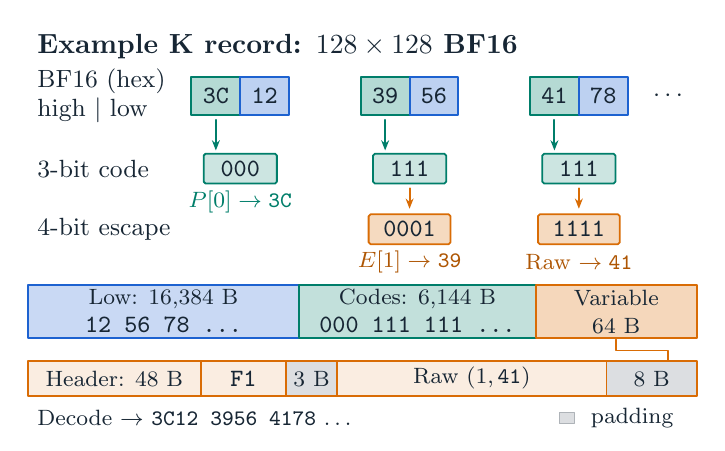
\begin{tikzpicture}[x=1cm,y=1cm,text=fpInk,
    font=\fontsize{9}{10.5}\selectfont,line cap=round,line join=round,
    arrow/.style={-{Stealth[length=1.3mm,width=1mm]},line width=.7pt},
    bits/.style={font=\fontsize{9}{10}\selectfont\ttfamily\bfseries},
    note/.style={font=\fontsize{8.5}{10}\selectfont}]
  \path[use as bounding box] (0,0) rectangle (8.5,5.02);
  \node[anchor=west,font=\fontsize{10}{11}\selectfont\bfseries]
    at (0,4.78) {Example K record: $128\times128$ BF16};

  % Three worked scalars: direct, extended-table and raw escape.
  \node[anchor=west,align=left] at (0,4.15) {BF16 (hex)\\high $\mid$ low};
  \foreach \x/\hi/\lo in {2.70/3C/12,4.85/39/56,7.00/41/78} {
    \draw[fpTeal,fill=fpTeal!29,line width=.7pt]
      (\x-.62,3.91) rectangle (\x,4.39);
    \draw[fpBlue,fill=fpBlue!29,line width=.7pt]
      (\x,3.91) rectangle (\x+.62,4.39);
    \node[bits] at (\x-.31,4.15) {\hi};
    \node[bits] at (\x+.31,4.15) {\lo};
    \draw[arrow,draw=fpTeal] (\x-.31,3.85) -- (\x-.31,3.46);
  }
  \node[bits] at (8.16,4.15) {$\cdots$};

  \node[anchor=west] at (0,3.23) {3-bit code};
  \foreach \x/\code in {2.70/000,4.85/111,7.00/111} {
    \node[draw=fpTeal,fill=fpTeal!20,line width=.65pt,
      rounded corners=.7pt,minimum width=.93cm,
      minimum height=.38cm,inner sep=1pt,bits] at (\x,3.23) {\code};
  }
  \node[note,text=fpTeal] at (2.70,2.81) {$P[0]\to\mathtt{3C}$};

  \node[anchor=west] at (0,2.46) {4-bit escape};
  \foreach \x/\nibble in {4.85/0001,7.00/1111} {
    \draw[arrow,draw=fpOrange] (\x,2.98) -- (\x,2.72);
    \node[draw=fpOrange,fill=fpOrange!25,line width=.65pt,
      rounded corners=.7pt,minimum width=1.04cm,
      minimum height=.38cm,inner sep=1pt,bits] at (\x,2.46) {\nibble};
  }
  \node[note,text=fpOrange!80!black] at (4.85,2.05) {$E[1]\to\mathtt{39}$};
  \node[note,text=fpOrange!80!black] at (7.00,2.05) {Raw $\to\mathtt{41}$};

  % Fixed streams show both size and corresponding example data in one band.
  \draw[fpBlue,fill=fpBlue!24,line width=.7pt]
    (0,1.08) rectangle (3.45,1.75);
  \draw[fpTeal,fill=fpTeal!24,line width=.7pt]
    (3.45,1.08) rectangle (6.45,1.75);
  \draw[fpOrange,fill=fpOrange!27,line width=.7pt]
    (6.45,1.08) rectangle (8.50,1.75);
  \node[note] at (1.725,1.57) {Low: 16,384 B};
  \node[note] at (4.95,1.57) {Codes: 6,144 B};
  \node[note,align=center] at (7.475,1.415) {Variable\\64 B};
  \node[bits] at (1.725,1.25) {12 56 78 \ldots};
  \node[bits] at (4.95,1.25) {000 111 111 \ldots};

  % Variable-detail pads retain their real byte counts without repeated prose.
  \draw[fpOrange,line width=.6pt] (7.475,1.06) -- (7.475,.92) -- (8.13,.92)
    -- (8.13,.79);
  \draw[fpOrange,fill=fpOrange!12,line width=.65pt]
    (0,.34) rectangle (8.50,.79);
  \fill[fpInk!15] (3.28,.35) rectangle (3.93,.78);
  \fill[fpInk!15] (7.35,.35) rectangle (8.49,.78);
  \foreach \x in {2.20,3.28,3.93,7.35}
    \draw[fpOrange,line width=.5pt] (\x,.34) -- (\x,.79);
  \node[note] at (1.10,.565) {Header: 48 B};
  \node[bits] at (2.74,.565) {F1};
  \node[note] at (3.605,.565) {3 B};
  \node[note] at (5.64,.565) {Raw $(1,\mathtt{41})$};
  \node[note] at (7.925,.565) {8 B};

  \node[anchor=west,note] at (0,.06)
    {Decode $\to$ \texttt{3C12 3956 4178} $\ldots$};
  \fill[fpInk!15,draw=fpInk!35,line width=.4pt] (6.75,-.01) rectangle (6.94,.13);
  \node[anchor=west,note] at (7.03,.06) {padding};
\end{tikzpicture}

\caption{Example of the FragPack record format using illustrative data
(not to scale). The three scalars show direct lookup, an extended-table
escape, and a raw escape. Each raw patch stores an escape's position in
the escape sequence and its original high byte. The variable region uses
64~B in this example, within the format's 2,048~B limit. Recombining the
high and low bytes recovers the original BF16 values exactly.}
\label{fig:record}
\end{figure}

A block's K and V records share a page within each layer. For four KV heads,
a page occupies 190,464~B instead of 262,144~B, allowing the same GPU budget
to hold 1.376 times as many pages before accounting for auxiliary backend
buffers. Records that exceed the encoding limit or do not fit in a shared
page are stored uncompressed in overflow slots. The reported token capacity
is calculated after reserving GPU memory for staging, overflow, and
workspaces.

\begin{samepage}
\subsection{Computing attention from compressed KV}
\emph{Prefill with gather + FA3.} When a request extends the context, the
adapter gathers the context's KV into a BF16 workspace, decoding compressed
records and copying values from open blocks. An unmodified FA3 kernel
computes attention from this workspace, which holds the current layer's KV.
Completed blocks remain compressed in each layer's pool.

\end{samepage}

\emph{Decode with fused attention.} For each generated token, a kernel divides
the request's context into page ranges, prefetches encoded records into
shared memory, and reconstructs operands in registers for tensor-core
attention. A final kernel combines partial softmax states across the
ranges. This path avoids writing the decoded context to GPU global memory
and supports decode-only CUDA graph replay. The backend is loaded through
vLLM's plugin interface and requires no changes to vLLM's source.

Both paths reconstruct the original KV bits exactly. Because the fused
kernel may use a different reduction order from FA3, the console displays
generated text separately from its KV byte checks.

\subsection{Storing KV in LMCache}
Once a block is complete, pool mode can save its attention records to
external storage for later reuse. An export kernel packs the records from
all layers into a relocatable blob that includes their dimensions, table
identity, and lengths. LMCache stores the blob at its actual length in
DRAM and NVMe. On import, the records are restored to GPU pages and their
record tables are updated. If validation fails, the load is rejected and
vLLM recomputes the KV. The cache server accesses worker pools through CUDA
IPC and launches export and import kernels on the corresponding GPU, with
one synchronization per load request. Each external chunk corresponds to
one 128-token engine block.

For deployments that keep the native GPU cache layout and attention
implementation, \emph{tier mode} compresses only the KV in external storage.
Each chunk contains one block's KV across all layers. Both modes share the
calibration procedure, with separate tables for K and V at each layer and
KV head. Tier records use the first 14 symbols of each table, seven primary
and seven secondary, while FragPack uses all 22. Values are stored in token
order. Escapes from the three-bit primary code lead to a second three-bit
code and, if needed, a literal high byte. Low bytes remain unchanged.
FragPack instead uses fragment order and four-bit escape selectors.
An index for each group of eight 256-scalar tiles stores base escape
counts and relative offsets to locate the escape streams. Codebooks are
fixed at startup and identified by a digest of the codec tables. Chunks
whose encoded size exceeds the raw storage limit are stored uncompressed.

Each tensor-parallel (TP) rank stores its own exact-length objects, aligned
to 4~KiB for NVMe direct I/O. After the step that produced the KV finishes,
the server encodes complete chunks directly from native pages into a bounded
GPU store pool. A separate worker synchronizes to read the encoded lengths,
allocates DRAM, copies the records, and commits them, leaving the load
thread free to serve requests. During a load, compressed records pass through a rotating set of
buffers and are decoded into destination pages. Raw records and partially
shared leading chunks are first restored into a scratch buffer, then
scattered into the destination pages. CUDA events coordinate copies,
decoding, and page reuse without host waits on the load path. LMCache
uses the stored lengths when prefetching objects from NVMe. Allocating
space for each object's encoded length lets the same budget retain more
session history.

\begin{figure*}[t]
\centering
% Actual Chromium captures of the current console, recorded mode, 2026-11-09.
% All image pixels come from unmodified DOM regions. No values are redrawn.
% Original capture provenance is summarized in evidence/README.md.
% Prefix: saved Qwen3-4B functional requests (2026-11-08).
% GPU and tier: historical Qwen3-30B AgentX comparisons (2026-11-04).
\begin{tikzpicture}[x=1cm,y=1cm,text=fpInk]
  \path[use as bounding box] (0,0) rectangle (17.8,7.65);
  \node[anchor=north west,inner sep=0,font=\footnotesize\bfseries]
    at (0,7.62) {(a) Extend a task};
  \node[anchor=north west,inner sep=0,font=\scriptsize,text=fpInk!75]
    at (0,7.23) {Recorded functional run};
  \node[anchor=north west,inner sep=0]
    at (0,6.84) {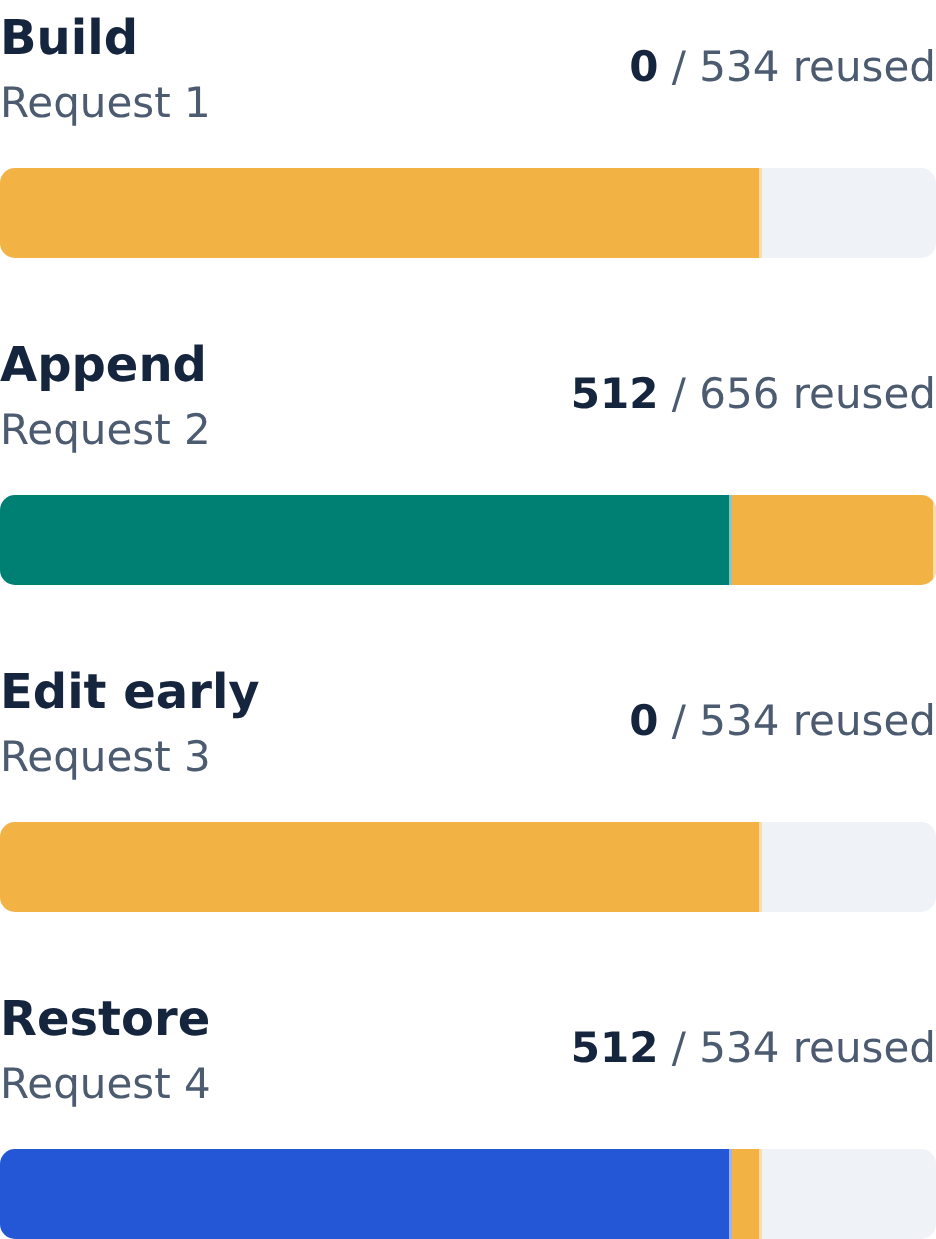
\includegraphics[width=5cm]{images/console-prefix(8).png}};
  \node[anchor=north west,inner sep=0,font=\footnotesize\bfseries]
    at (5.25,7.62) {(b) Add sessions};
  \node[anchor=north west,inner sep=0,font=\scriptsize,text=fpInk!75]
    at (5.25,7.23) {Recorded benchmark: $S=12$};
  \node[anchor=north west,inner sep=0]
    at (5.25,6.84) {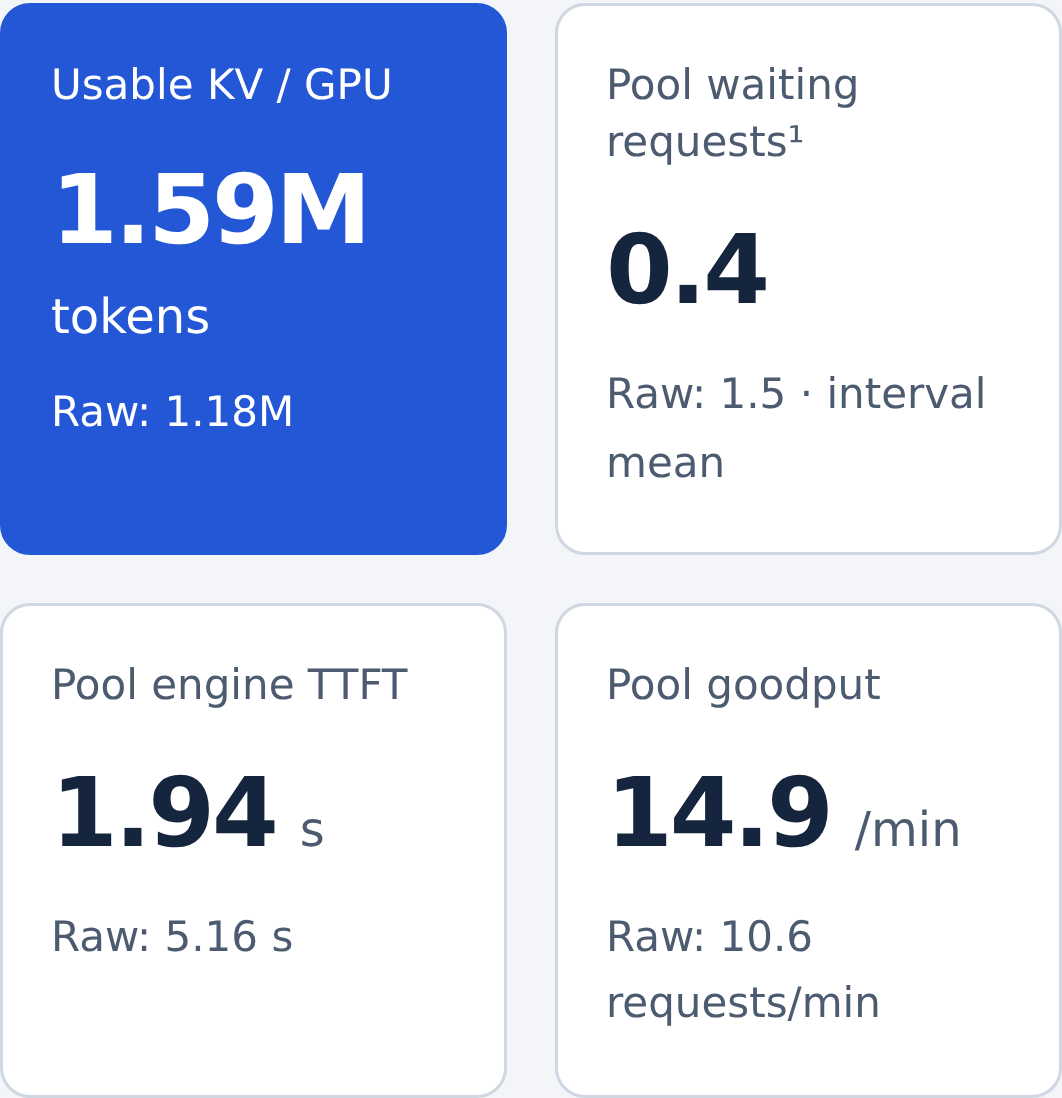
\includegraphics[width=6.15cm]{images/console-gpu(8).png}};
  \node[anchor=north west,inner sep=0,font=\footnotesize\bfseries]
    at (11.65,7.62) {(c) Revisit history};
  \node[anchor=north west,inner sep=0,font=\scriptsize,text=fpInk!75]
    at (11.65,7.23) {Recorded benchmark: 640 GiB NVMe};
  \node[anchor=north west,inner sep=0]
    at (11.65,6.84) {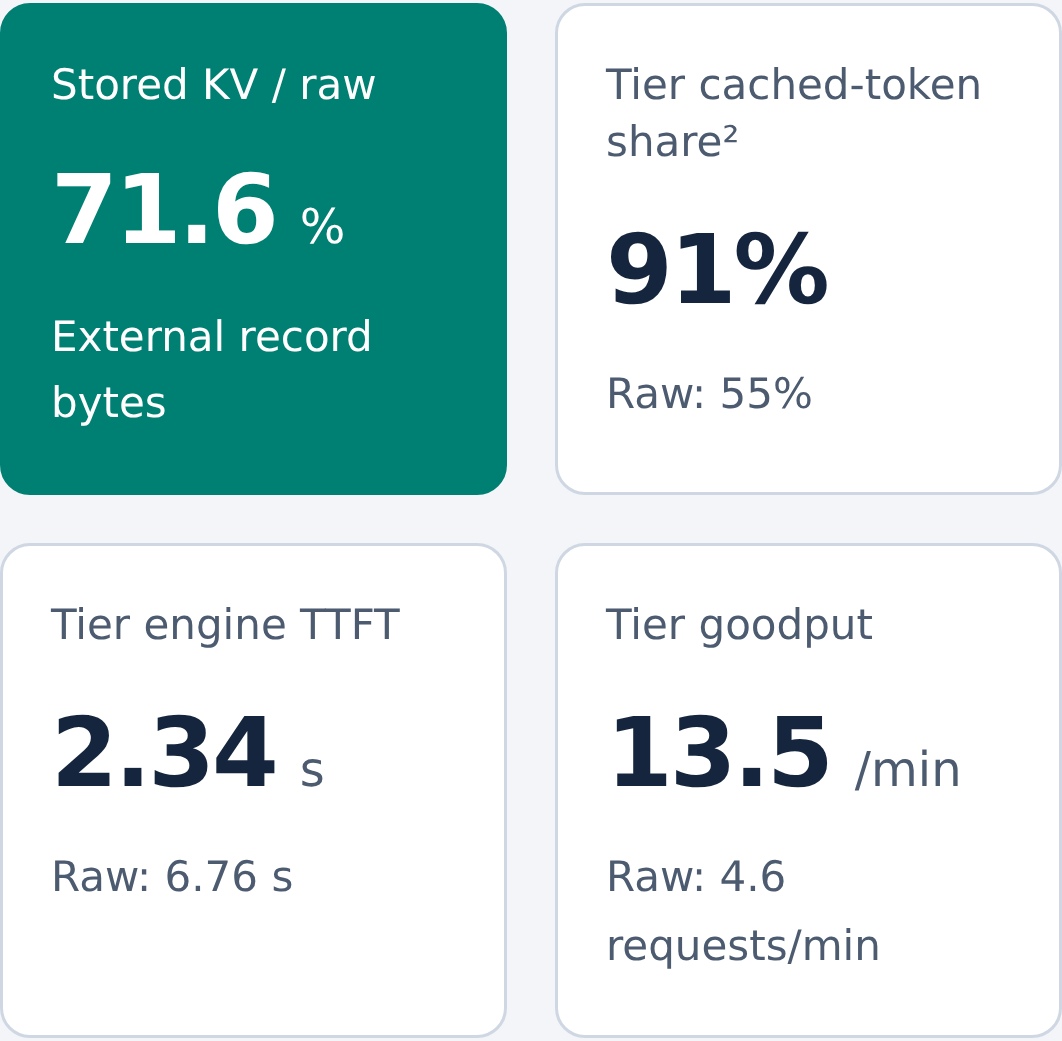
\includegraphics[width=6.15cm]{images/console-tier(8).png}};
\end{tikzpicture}

\caption{Screenshots of the implemented console. Left: a saved Qwen3-4B
prefix-reuse session. Center and right: recorded GPU-capacity and
external-capacity comparisons from Tables~\ref{tab:gpu} and~\ref{tab:tiers},
measured separately with Qwen3-30B-A3B. Superscripts denote $^{1}$mean waiting
requests and $^{2}$the combined GPU/external cached-token share.}
\label{fig:views}
\end{figure*}

\section{Demonstration}
\label{sec:demo}
Visitors follow the timeout investigation through prefix reuse, GPU
pressure, and returning sessions (Figure~\ref{fig:views}). The console
identifies live and recorded data, model, TP degree, KV type, mode, and
budgets. Modes and codebooks are fixed at startup; selectors change the
displayed records. Offline, the saved session remains viewable with request
controls disabled.

\emph{Setup.} The interactive session uses Qwen3-4B-Instruct-2507 with BF16
weights and KV, TP 1, and one H800 PCIe GPU. It uses eager execution in pool
mode, with 128-token blocks, a 4~GiB GPU KV budget, and 1~GiB of LMCache DRAM.

The recorded capacity experiments used Qwen3-30B-A3B-Instruct
with FP8 weights and BF16 KV, TP 2, and two H800 SXM GPUs connected over
PCIe. vLLM used 128-token blocks and 8,192-token chunked prefill.
AgentX harness 1.0.7 replayed \texttt{cc\_traces\_weka\_062126\_256k} with
seed 42 and recorded think times. $P$ counts live root sessions; a FIFO
proxy admits at most $S$ concurrent requests. Measurements covered
1,800 seconds after priming and ten warmup requests, excluding requests
without a first token by the window's end. \emph{Engine TTFT} excludes
proxy wait. \emph{Goodput} counts requests/minute with engine TTFT at most
2~s and inter-token latency (ITL) at most 40~ms.

% Current codec description: feat/lmcache-056-lossless-kv at d096273.
% Recorded measurements: main(11).pdf, November 4, 2026; exact run commits
% are not identified in the supplied report.
These measurements and output checks predate the shared calibration and
grouped index described in Section~\ref{sec:design}. The recorded tier runs
used per-plane codebooks and the earlier tile index.

\subsection{Step 1: extend a task and inspect prefix reuse}
With repository context and a bug report loaded, visitors use \emph{Build}
to submit ``Diagnose the timeout failure.'' They can then \emph{Append} the
request ``Write a regression test.'' A prefix strip summarizes reused and newly
computed tokens alongside the engine's cached-token count, TTFT, and
continuation. \emph{Edit early} changes an early token, limiting reuse to
complete 128-token blocks before the edit.

\emph{Restore} waits for external saves, resets the GPU prefix cache, and
replays the original prompt. The console reports the source and token
counts: in the captured session, LMCache restored 512 tokens from CPU DRAM.

The inspector compares decoded KV from an already encoded block before
and after export through host memory and import into an independent GPU
scratch store. All layers of the captured 128-token block matched byte for
byte. It displays sizes, checksums, and mismatch counts. Separate CPU
reference samples exercise escapes and raw fallback.

A separate historical output check found identical greedy outputs for
192 repeat-trace requests in tier and raw-tier modes with matching execution
paths.

\subsection{Step 2: explore GPU capacity limits}
Visitors switch between $S=8$ and $S=12$ to compare raw and pool modes
under equal GPU KV budgets (Table~\ref{tab:gpu}). The external tiers retain
the working set, with cached-token share fixed at 0.94. These runs examine
GPU pressure when prefixes are already cached.

% Source: main(11).pdf, p.10, Table V; printed values retained verbatim.
\begin{table}[t]
\centering
\caption{GPU capacity and performance in the recorded runs: 54 GiB KV per
GPU, $P=64$, 400 GiB DRAM, and 2 TiB NVMe. Wait denotes the mean number of
requests waiting in vLLM; TTFT is mean engine TTFT in seconds.}
\label{tab:gpu}
\small
\setlength{\tabcolsep}{3pt}
\begin{tabular*}{\columnwidth}{@{\extracolsep{\fill}}rlrrrr@{}}
\toprule
$S$ & Mode & KV tokens & Wait & TTFT & Goodput \\
\midrule
8  & Raw  & 1.18M & 0.3 & 1.69 & 15.1 \\
8  & Pool & 1.59M & 0.2 & 1.34 & 16.2 \\
12 & Raw  & 1.18M & 1.5 & 5.16 & 10.6 \\
12 & Pool & 1.59M & 0.4 & 1.94 & 14.9 \\
\bottomrule
\end{tabular*}
\end{table}

Pool mode reserves 1.3~GiB within the KV budget for staging, overflow, and
the prefill workspace. Cache-server CUDA contexts and transfer buffers are
accounted for separately; codec buffers occupy 1.0~GiB per GPU outside
vLLM's budget.

At $S=12$, pool mode keeps TTFT close to the raw baseline at $S=8$,
while reducing waiting requests and increasing goodput at the same
admission cap. The console places these changes beside usable KV capacity.

\subsection{Step 3: revisit sessions under storage pressure}
Visitors switch between 640~GiB and 2~TiB NVMe to compare retained
history, stored bytes, TTFT, and goodput (Table~\ref{tab:tiers}). Raw and tier
modes use the same native GPU KV layout, FA3, and LMCache LRU, write-through,
and prefetch policies; the allocated record sizes differ.

% Source: main(11).pdf, p.9, Table III; same P/S and metric definitions.
\begin{table}[t]
\centering
\caption{External cache capacity and performance in the recorded runs:
$P=64$, $S=8$, and 400 GiB DRAM. Cached denotes the share of prompt tokens
served from the GPU or external cache; TTFT is mean engine TTFT in seconds.}
\label{tab:tiers}
\small
\setlength{\tabcolsep}{3pt}
\begin{tabular*}{\columnwidth}{@{\extracolsep{\fill}}llrrr@{}}
\toprule
NVMe & Mode & Cached & TTFT & Goodput \\
\midrule
640 GiB & Raw  & 0.55 & 6.76 & 4.6 \\
640 GiB & Tier & 0.91 & 2.34 & 13.5 \\
2 TiB   & Raw  & 0.94 & 1.69 & 15.1 \\
2 TiB   & Tier & 0.94 & 1.85 & 15.4 \\
\bottomrule
\end{tabular*}
\end{table}

With 640~GiB of NVMe, tier mode retains more prefixes for returning
sessions (Table~\ref{tab:tiers}). Its compressed-to-raw size ratio of
0.716 allows the same storage capacity to hold about 1.4 times as much
KV. With 2~TiB, the uncompressed working set already fits, so the
cached-token shares converge. In this case, compression adds overhead:
input throughput is 26.9 thousand tokens/s in tier mode, compared with
27.5 for raw storage, a 2.2\% reduction.

A separate experiment replayed 48 prompts with one request in flight at a
time to compare DRAM hits with NVMe hits. The KV occupies 261~GiB
uncompressed and 188~GiB compressed. With 220~GiB of DRAM, the compressed
working set fits entirely in memory, while some uncompressed prefixes
must be loaded from NVMe. Across the recorded 8K--128K prompts, mean warm
TTFT for raw storage is 1.63--1.68 times that of tier mode. Both working
sets fit in 400~GiB of DRAM, where the latency gap narrows. Selecting this
trace displays static comparisons of recorded residency and latency.
Showing a transfer timeline would require additional time-series
measurements.

\section{Conclusion}
KVFold fits more KV into GPU memory and external cache tiers. Visitors
inspect prefix reuse, restore KV from LMCache, and check a model block
before and after transfer. Recorded comparisons show how the additional
capacity affects request queues and history reuse under fixed budgets.

\section*{Acknowledgment}
OpenAI Codex assisted with drafting and figure preparation. Experimental
values were taken from the authors' recorded results.

\bibliographystyle{IEEEtran}
\bibliography{references}
\end{document}
